\documentclass[12pt]{article}

\usepackage{setspace}
\usepackage{graphicx}
\usepackage{float}
\usepackage{amsmath}

\onehalfspacing

\begin{document}

%------------------------------------------------
% TITLE PAGE
%------------------------------------------------

\begin{titlepage}
\begin{center}

\vspace*{2cm}

{\Large \textbf{M.Tech Project Report (Phase - 1)}}

{\large on}

{\Large \textbf{Financial Market Volatility Prediction using}}

{\Large \textbf{Machine Learning and Transformer Models}}

\vspace{2cm}

Submitted by

{\Large \textbf{Dhayal SR}}\

(Reg. Number: 21MDA044)

\vspace{1cm}

Under the guidance of\

\textbf{Dr. Utkarsh Khaire}

\vspace{0.5cm}

Project Guide\

\textbf{Vimal Shanmuganathan}

\vspace{2cm}


\includegraphics[width=0.45\textwidth]{iiIT-Dharwad-Logo-horizontal-500x154[1].png}

\vspace{1cm}

\textbf{DEPARTMENT OF COMPUTER SCIENCE AND ENGINEERING}

\textbf{INDIAN INSTITUTE OF INFORMATION TECHNOLOGY DHARWAD}

\textbf{2024--2025}

\end{center}
\end{titlepage}


%------------------------------------------------
% DECLARATION
%------------------------------------------------

\newpage
\section*{Declaration}

I declare that this report titled \textbf{Financial Market Volatility Prediction using Machine Learning and Transformer Models} is my original work carried out under the supervision of \textbf{Dr. Utkarsh Khaire}.

\vspace{2cm}

Place: Dharwad

Date:

\vspace{1cm}

Signature: Dhayal SR

%------------------------------------------------
% ABSTRACT
%------------------------------------------------

\newpage
\section*{Abstract}

Financial markets are complex systems influenced by economic and behavioral factors. Predicting financial market volatility is important for portfolio management, risk assessment and algorithmic trading.

This project explores machine learning and deep learning techniques for predicting financial market volatility. Historical NIFTY ETF price data is combined with macroeconomic indicators including inflation rate, GDP growth rate and India VIX volatility index.

Technical indicators such as Moving Average, Relative Strength Index (RSI), Momentum and MACD are computed to enhance the dataset.

Machine learning models such as Linear Regression and Random Forest are used as baseline models, while deep learning architectures including Long Short-Term Memory networks and Transformer models are proposed for improved financial forecasting.

This Phase-1 report focuses on literature review, identification of research gaps and the design of the proposed methodology.

%------------------------------------------------
% CONTENTS
%------------------------------------------------

\newpage
\tableofcontents

%------------------------------------------------
% INTRODUCTION
%------------------------------------------------

\newpage
\section{Introduction}

Financial markets are dynamic and influenced by several economic indicators and investor behavior. Predicting financial market volatility helps investors manage risk and improve investment decisions.

Traditional statistical models such as ARIMA and GARCH have been widely used in financial forecasting. However, these models often struggle to capture nonlinear relationships present in financial time series.

Machine learning and deep learning models provide powerful tools for modeling complex financial data. Neural networks and Transformer models have shown strong performance in sequence modeling tasks.

The objectives of this project are:

\begin{itemize}

\item Collect financial and macroeconomic datasets

\item Perform data preprocessing

\item Generate technical indicators

\item Implement machine learning models

\item Implement deep learning models such as LSTM and Transformer

\end{itemize}

%------------------------------------------------
% LITERATURE REVIEW
%------------------------------------------------

\newpage
\section{Literature Review}

Several studies have explored machine learning and deep learning techniques for financial forecasting.

Support Vector Machines were among the earliest machine learning methods used for stock market prediction.

Long Short-Term Memory networks have demonstrated strong performance for modeling sequential financial data.

Transformer architectures introduced attention mechanisms that enable models to capture long-range dependencies in time series data.

These advancements have opened new opportunities for improving financial market prediction accuracy.

%------------------------------------------------
% RESEARCH GAP
%------------------------------------------------

\newpage
\section{Research Gap}

Most existing research focuses primarily on historical stock price data while ignoring macroeconomic indicators.

Additionally, limited studies compare traditional machine learning models with modern Transformer architectures for volatility prediction.

This project aims to integrate macroeconomic variables with financial data and evaluate the effectiveness of machine learning and Transformer-based models.

%------------------------------------------------
% PROPOSED METHODOLOGY
%------------------------------------------------

\newpage
\section{Proposed Methodology}

The proposed framework consists of multiple stages including data collection, preprocessing, feature engineering and model training.

\begin{figure}[H]
\centering
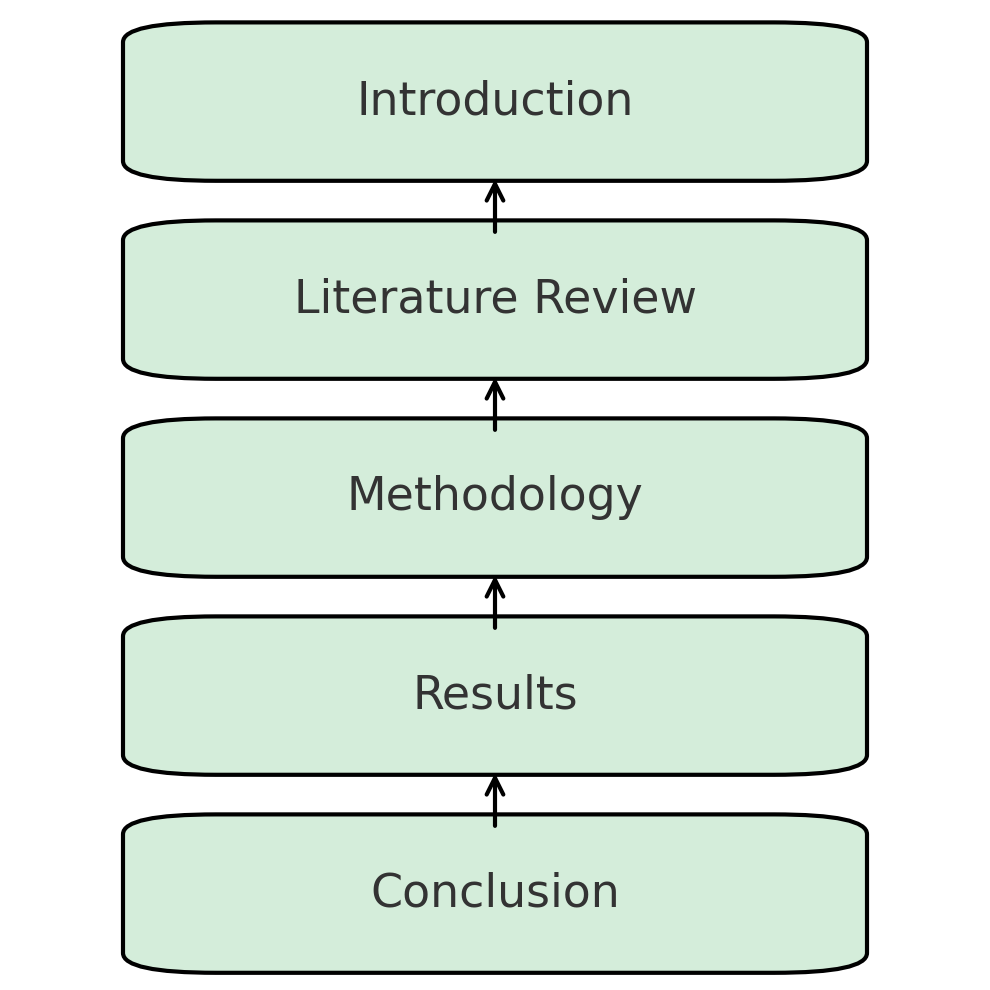
\includegraphics[width=0.7\textwidth]{simple_project_report_flow.png}
\caption{Proposed System Architecture}
\end{figure}

%------------------------------------------------
% MODEL EQUATIONS
%------------------------------------------------

\newpage
\section{Model Formulation}

LSTM models capture temporal dependencies in time-series data.

\begin{equation}
h_t = f(Wx_t + Uh_{t-1} + b)
\end{equation}

Transformer models use attention mechanisms defined as:

\begin{equation}
Attention(Q,K,V) = softmax\left(\frac{QK^T}{\sqrt{d_k}}\right)V
\end{equation}

%------------------------------------------------
% DATASET
%------------------------------------------------

\newpage
\section{Dataset}

The dataset used in this project includes:

\begin{itemize}

\item Historical NIFTY ETF price data

\item India VIX volatility index

\item Inflation rate

\item GDP growth rate

\end{itemize}

Technical indicators used include:

\begin{itemize}

\item Moving Average

\item Relative Strength Index

\item Momentum

\item MACD

\end{itemize}

%------------------------------------------------
% EXPECTED OUTCOME
%------------------------------------------------

\newpage
\section{Expected Outcome}

The expected outcome of this project is a predictive framework capable of forecasting financial market volatility using machine learning and deep learning models.

%------------------------------------------------
% CONCLUSION
%------------------------------------------------

\newpage
\section{Conclusion}

This Phase-1 report presented the background, literature review and proposed methodology for financial market volatility prediction.

Future work will involve implementing deep learning models and evaluating their predictive performance.

%------------------------------------------------
% REFERENCES
%------------------------------------------------

\newpage
\section*{References}

1. Fischer, T., Krauss, C. Deep learning with LSTM networks for financial prediction.

2. Vaswani, A. et al. Attention Is All You Need.

3. Bao, W., Yue, J., Rao, Y. Deep learning framework for financial forecasting.

4. Kim, K. Financial forecasting using support vector machines.

5. Gu, S., Kelly, B., Xiu, D. Machine learning in asset pricing.

\end{document}
